\documentclass[11pt]{article}
\newcommand{\doctitle}{PIC — Design Specification}
\newcommand{\docsubject}{Programmable interrupt controller · interface and register contract}
\newcommand{\docrev}{2.2}
\newcommand{\docdate}{23 September 2026}
% ---------------------------------------------------------------------------
% Shared preamble for the specification set.
% Compiled with LuaLaTeX.
% ---------------------------------------------------------------------------
\usepackage{fontspec}
\setmainfont{Latin Modern Roman}[SmallCapsFont={Latin Modern Roman Caps}]
\setsansfont{Latin Modern Sans}
\setmonofont{Latin Modern Mono}[BoldFont={Latin Modern Mono}]

\usepackage[a4paper,top=27mm,bottom=25mm,left=25mm,right=22mm,headheight=15pt]{geometry}

\usepackage{amsmath}
\usepackage{amssymb}
\usepackage{booktabs}
\usepackage{longtable}
\usepackage{tabularx}
\usepackage{array}
\usepackage{multirow}
\usepackage{enumitem}
\usepackage{xcolor}
\usepackage{fancyhdr}
\usepackage{titlesec}
\usepackage{caption}
\usepackage{float}
\usepackage{graphicx}
\usepackage{tikz}
\usepackage{tikz-timing}
\usetikzlibrary{arrows.meta,positioning,automata,calc,fit,backgrounds,
                shapes.geometric,shapes.misc,decorations.pathreplacing}
\usepackage[hidelinks,bookmarksnumbered]{hyperref}

% --- palette ---------------------------------------------------------------
\definecolor{accent}{RGB}{0,72,110}
\definecolor{rulegrey}{RGB}{120,120,120}
\definecolor{boxbg}{RGB}{244,246,248}

% --- head / foot -----------------------------------------------------------
\pagestyle{fancy}
\fancyhf{}
\fancyhead[L]{\small\nouppercase{\leftmark}}
\fancyhead[R]{\small\thepage}
\fancyfoot[L]{\footnotesize\doctitle}
\fancyfoot[R]{\footnotesize Rev.\ \docrev\ --- \docdate}
\renewcommand{\headrulewidth}{0.4pt}
\renewcommand{\footrulewidth}{0.4pt}
\fancypagestyle{plain}{%
  \fancyhf{}%
  \fancyfoot[L]{\footnotesize\doctitle}%
  \fancyfoot[R]{\footnotesize Rev.\ \docrev\ --- \docdate}%
  \renewcommand{\headrulewidth}{0pt}%
  \renewcommand{\footrulewidth}{0.4pt}%
}

\titleformat{\section}{\normalfont\Large\bfseries\color{accent}}{\thesection}{0.7em}{}
\titleformat{\subsection}{\normalfont\large\bfseries}{\thesubsection}{0.7em}{}
\titleformat{\subsubsection}{\normalfont\normalsize\bfseries}{\thesubsubsection}{0.7em}{}
\titlespacing*{\section}{0pt}{16pt}{8pt}

\captionsetup{font=small,labelfont={bf,color=accent},skip=5pt}
\setcounter{secnumdepth}{3}
\setcounter{tocdepth}{3}

% --- macros ----------------------------------------------------------------
\newcommand{\sig}[1]{\texttt{#1}}
\newcommand{\reg}[1]{\texttt{#1}}

\newcolumntype{L}[1]{>{\raggedright\arraybackslash}p{#1}}
\newcolumntype{C}[1]{>{\centering\arraybackslash}p{#1}}

\tikzset{
  blk/.style={draw=accent,fill=white,rounded corners=1.5pt,align=center,
              inner sep=5pt,font=\small,minimum height=9mm},
  blkf/.style={blk,fill=boxbg},
  regbox/.style={draw=rulegrey,fill=boxbg,align=center,inner sep=4pt,font=\footnotesize},
  flow/.style={-{Stealth[length=2.4mm]},thick,draw=accent},
  flowd/.style={flow,dashed},
  lbl/.style={font=\scriptsize,inner sep=1.5pt,fill=white},
  stb/.style={draw=accent,fill=white,rounded corners=2pt,align=center,
              font=\small,inner xsep=5pt,inner ysep=4pt,
              minimum height=8mm,minimum width=19mm},
  stbi/.style={stb,double,double distance=0.6pt},
}

% identification block used on the title page of every document in the set
\providecommand{\docsubject}{}
\newcommand{\identblock}[1]{%
\begin{center}
\begin{tabular}{@{}L{0.28\linewidth}L{0.60\linewidth}@{}}
\toprule
Document & \doctitle \\
Document type & #1 \\
Subject & \docsubject \\
Revision & \docrev \\
Date & \docdate \\
Author & Bunea Cosmin-Andrei \\
Status & Released for review \\
\bottomrule
\end{tabular}
\end{center}}

\begin{document}
\begin{titlepage}\vspace*{24mm}
{\Huge\bfseries\color{accent}PIC\par}\vspace{4mm}{\LARGE Design Specification\par}\vspace{12mm}
{\Large Programmable interrupt controller · interface and register contract\par}\vfill
\identblock{Design specification}\end{titlepage}
\tableofcontents
\clearpage
\section{Introduction}

\needspace{7\baselineskip}
\subsection{Purpose of the document}
\noindent This specification describes the implemented RTL, programming model and integration contracts of the programmable interrupt controller. It is intended for hardware designers, verification engineers and software developers integrating the block.\par\medskip
\noindent It defines the behaviour that the RTL must show at its interfaces.\par\medskip

\needspace{7\baselineskip}
\subsection{Validity of the document}
\noindent The documented configuration is the RTL in cpu/hdl and the associated CPU/PIC and SoC simulation environments. Interface adaptations from the supplied briefs are identified in the integration section.\par\medskip
\noindent Revision 2.2 of 23 September 2026 describes the delivered state of that RTL.\par\medskip

\needspace{7\baselineskip}
\subsection{Definitions of terms and abbreviations}
{\small
\begin{longtable}{@{}L{0.2300\dimexpr\linewidth-12pt\relax}L{0.7700\dimexpr\linewidth-12pt\relax}@{}}
\toprule
\textbf{Term} & \textbf{Meaning} \\ \midrule
\endfirsthead
\toprule
\textbf{Term} & \textbf{Meaning} \\ \midrule
\endhead
AXI4-Lite & Single-beat AXI read/write channels. \\ \addlinespace[3pt]
CSR & Control and status register. \\ \addlinespace[3pt]
DUT & Device under test. \\ \addlinespace[3pt]
EOI & End of interrupt; completes one service level. \\ \addlinespace[3pt]
IRQ & Interrupt request. \\ \addlinespace[3pt]
NBA & Nonblocking-assignment update region in simulation. \\ \addlinespace[3pt]
PIC & Programmable interrupt controller. \\ \addlinespace[3pt]
SVA & SystemVerilog Assertions. \\*
\bottomrule\end{longtable}}

\needspace{7\baselineskip}
\subsection{Relationship with other documents}
\noindent The documents below are the ones this specification is derived from or read with.\par\medskip
{\small
\begin{longtable}{@{}L{0.3400\dimexpr\linewidth-36pt\relax}L{0.2200\dimexpr\linewidth-36pt\relax}L{0.1800\dimexpr\linewidth-36pt\relax}L{0.2600\dimexpr\linewidth-36pt\relax}@{}}
\toprule
\textbf{Document} & \textbf{Version / date} & \textbf{Author} & \textbf{Relationship} \\ \midrule
\endfirsthead
\toprule
\textbf{Document} & \textbf{Version / date} & \textbf{Author} & \textbf{Relationship} \\ \midrule
\endhead
Programmable Interrupt Controller with Advanced Scheduling & Draft, 26 June 2026 & D. Borzasi, Siemens & Functional requirements; see section 2. \\ \addlinespace[3pt]
Spec table of contents and templates & 2 September 2026 & D. Borzasi, Siemens & Document structure and verification-plan template. \\ \addlinespace[3pt]
Verification Specification — PIC & Rev. 2.2, 23 September 2026 & C.-A. Bunea & Companion document. \\ \addlinespace[3pt]
Design Specification — RV32I CPU & Rev. 2.2, 23 September 2026 & C.-A. Bunea & Other side of the CPU–PIC interrupt link. \\ \addlinespace[3pt]
AMBA AXI and ACE Protocol Specification & IHI0022E & Arm & AXI4-Lite ports. \\ \addlinespace[3pt]
IEEE Std 1364 (Verilog) & 2005 & IEEE & RTL language. \\*
\bottomrule\end{longtable}}

\needspace{7\baselineskip}
\subsection{Notes on the notation used}
\noindent Signal and register names follow the RTL. Addresses and waveform bus values are hexadecimal; time is in ns and widths are in bits. Register offsets are byte offsets; CSR addresses are instruction-encoded indices.\par\medskip
{\small
\begin{longtable}{@{}L{0.2600\dimexpr\linewidth-12pt\relax}L{0.7400\dimexpr\linewidth-12pt\relax}@{}}
\toprule
\textbf{Notation} & \textbf{Meaning} \\ \midrule
\endfirsthead
\toprule
\textbf{Notation} & \textbf{Meaning} \\ \midrule
\endhead
Fixed-width name & A Verilog module, port, file or script name, spelled as in the source. \\ \addlinespace[3pt]
Signal suffix \_i / \_o & Module input / output, seen from inside that module. \\ \addlinespace[3pt]
[a:b] & Bit range, most significant bit first. \\ \addlinespace[3pt]
Source slot & One of the 16 arbitration identities; x or n denotes its index 0–15. \\ \addlinespace[3pt]
posedge +1 ns & A testbench stimulus time, one nanosecond after the sampling edge. \\*
\bottomrule\end{longtable}}

\clearpage
\section{Specifications and system integration}
\subsection{Requirements and integration}
\noindent The table sets each requirement of the brief Programmable Interrupt Controller with Advanced Scheduling against the contract implemented in pic.v and axi\_lite\_slave.v. In the SoC, the register port sits on the CPU data decoder; sources 0–3 are the DMA channels, 4 the SRAM and 7 the timer, and the remaining inputs are tied low.\par\medskip
{\small
\begin{longtable}{@{}L{0.1500\dimexpr\linewidth-24pt\relax}L{0.3500\dimexpr\linewidth-24pt\relax}L{0.5000\dimexpr\linewidth-24pt\relax}@{}}
\toprule
\textbf{Topic} & \textbf{Initial requirement} & \textbf{Implemented contract} \\ \midrule
\endfirsthead
\toprule
\textbf{Topic} & \textbf{Initial requirement} & \textbf{Implemented contract} \\ \midrule
\endhead
Sources & 16 hardware lines and 16 software-trigger channels. & HW/SW merge into 16 source slots; one vector per slot. \\ \addlinespace[3pt]
Priority grouping & Define bands and inter-/intra-band arbitration. & Four bands; programmable 2-bit urgency; 4-bit intra-band priority; lowest ID breaks ties. \\ \addlinespace[3pt]
Preemption & Preserve and restore active contexts. & 16-entry stack; configured limit 1–16, reset 8; explicit EOI pops one level. \\ \addlinespace[3pt]
Spurious requests & Detect a source withdrawn before acknowledgement. & Claim-time detection; source and global sticky logs. \\ \addlinespace[3pt]
Deadlines & Per-source service deadline and automatic escalation. & 16-bit cycle count; jump or next-more-urgent-band policy; optional repeated escalation. \\ \addlinespace[3pt]
Software trigger & Protect injection; define clear and HW/SW collision. & 0xA5A5 key; key byte strobes required; zero or claim clears request. \\ \addlinespace[3pt]
Register port & AXI4-Lite slave; documented register map. & 32-bit data/address; 256-byte window; independent AW/W collection. \\ \addlinespace[3pt]
Reset / target & Active-low asynchronous reset; behavioural RTL simulation. & posedge clk\_i; reset disables all sources; no synthesis result claimed. \\*
\bottomrule\end{longtable}}

\needspace{7\baselineskip}
\subsection{Configuration and integration limits}
\noindent The module has no Verilog parameters: every quantity is either fixed in the RTL or programmed through a register. The first table lists the fixed quantities; the second states what an integrator has to guarantee outside the block.\par\medskip
{\small
\begin{longtable}{@{}L{0.3500\dimexpr\linewidth-12pt\relax}L{0.6500\dimexpr\linewidth-12pt\relax}@{}}
\toprule
\textbf{Fixed quantity} & \textbf{Value} \\ \midrule
\endfirsthead
\toprule
\textbf{Fixed quantity} & \textbf{Value} \\ \midrule
\endhead
Source slots & 16; each merges a hardware line and software request. \\ \addlinespace[3pt]
Priority bands & 4; configurable urgency, not additional modules. \\ \addlinespace[3pt]
Physical nesting depth & 16; run-time NEST\_MAX defaults to 8. \\ \addlinespace[3pt]
AXI width & 32-bit address/data; four strobes; three protection bits; two response bits. \\*
\bottomrule\end{longtable}}
{\small
\begin{longtable}{@{}L{0.2600\dimexpr\linewidth-12pt\relax}L{0.7400\dimexpr\linewidth-12pt\relax}@{}}
\toprule
\textbf{Constraint} & \textbf{Required integration behaviour} \\ \midrule
\endfirsthead
\toprule
\textbf{Constraint} & \textbf{Required integration behaviour} \\ \midrule
\endhead
Address window & Decode exactly a 256-byte window. Only address bits [7:2] are used; upper bits alias and low bits select the containing word. \\ \addlinespace[3pt]
IRQ input synchrony & irq\_src\_i must be synchronous to clk\_i; synchronize asynchronous peripheral sources outside the PIC. \\ \addlinespace[3pt]
CPU handshake & Claim refers to the offer sampled one cycle earlier. Never assert claim and EOI together. \\ \addlinespace[3pt]
One CPU & One offer / mask / claim / EOI interface per PIC instance. \\ \addlinespace[3pt]
Protection & AWPROT/ARPROT accepted and ignored; no access-control mechanism in this block. \\ \addlinespace[3pt]
Implementation target & Behavioural RTL simulation. No synthesis / frequency claim. \\*
\bottomrule\end{longtable}}

\needspace{7\baselineskip}
\subsection{Interface adaptations}
\noindent The integrated CPU/PIC interface resolves the different source counts in the two drafts. The following choices define the implemented connection and arbitration timing.\par\medskip
{\small
\begin{longtable}{@{}L{0.3400\dimexpr\linewidth-12pt\relax}L{0.6600\dimexpr\linewidth-12pt\relax}@{}}
\toprule
\textbf{Brief item} & \textbf{Implemented contract} \\ \midrule
\endfirsthead
\toprule
\textbf{Brief item} & \textbf{Implemented contract} \\ \midrule
\endhead
CPU brief IRQ interface & 8 request bits / 3-bit ID / 8 acknowledge bits become one offer, 4-bit source ID, 16-bit pending/mask and scalar claim/EOI. \\ \addlinespace[3pt]
Claim / completion & Claim starts active service and consumes latched requests. The added EOI input completes service and pops one context. \\ \addlinespace[3pt]
Resolution pipeline & The PIC brief describes staged resolution. This RTL resolves eligibility and the priority key combinationally and registers the offer; there are no successive registered arbitration stages. \\*
\bottomrule\end{longtable}}

\clearpage
\newgeometry{top=15mm,bottom=15mm,left=16mm,right=16mm}
\begin{landscape}
\thispagestyle{plain}
\section{Overview of overall structure}

\noindent An enabled HW or software request enters priority selection. The registered offer identifies the candidate; claim saves its ID and priority, while EOI restores the previous active context. The return paths carry masks, the saved priority threshold and the depth limit.\par
\begin{figure}[H]\centering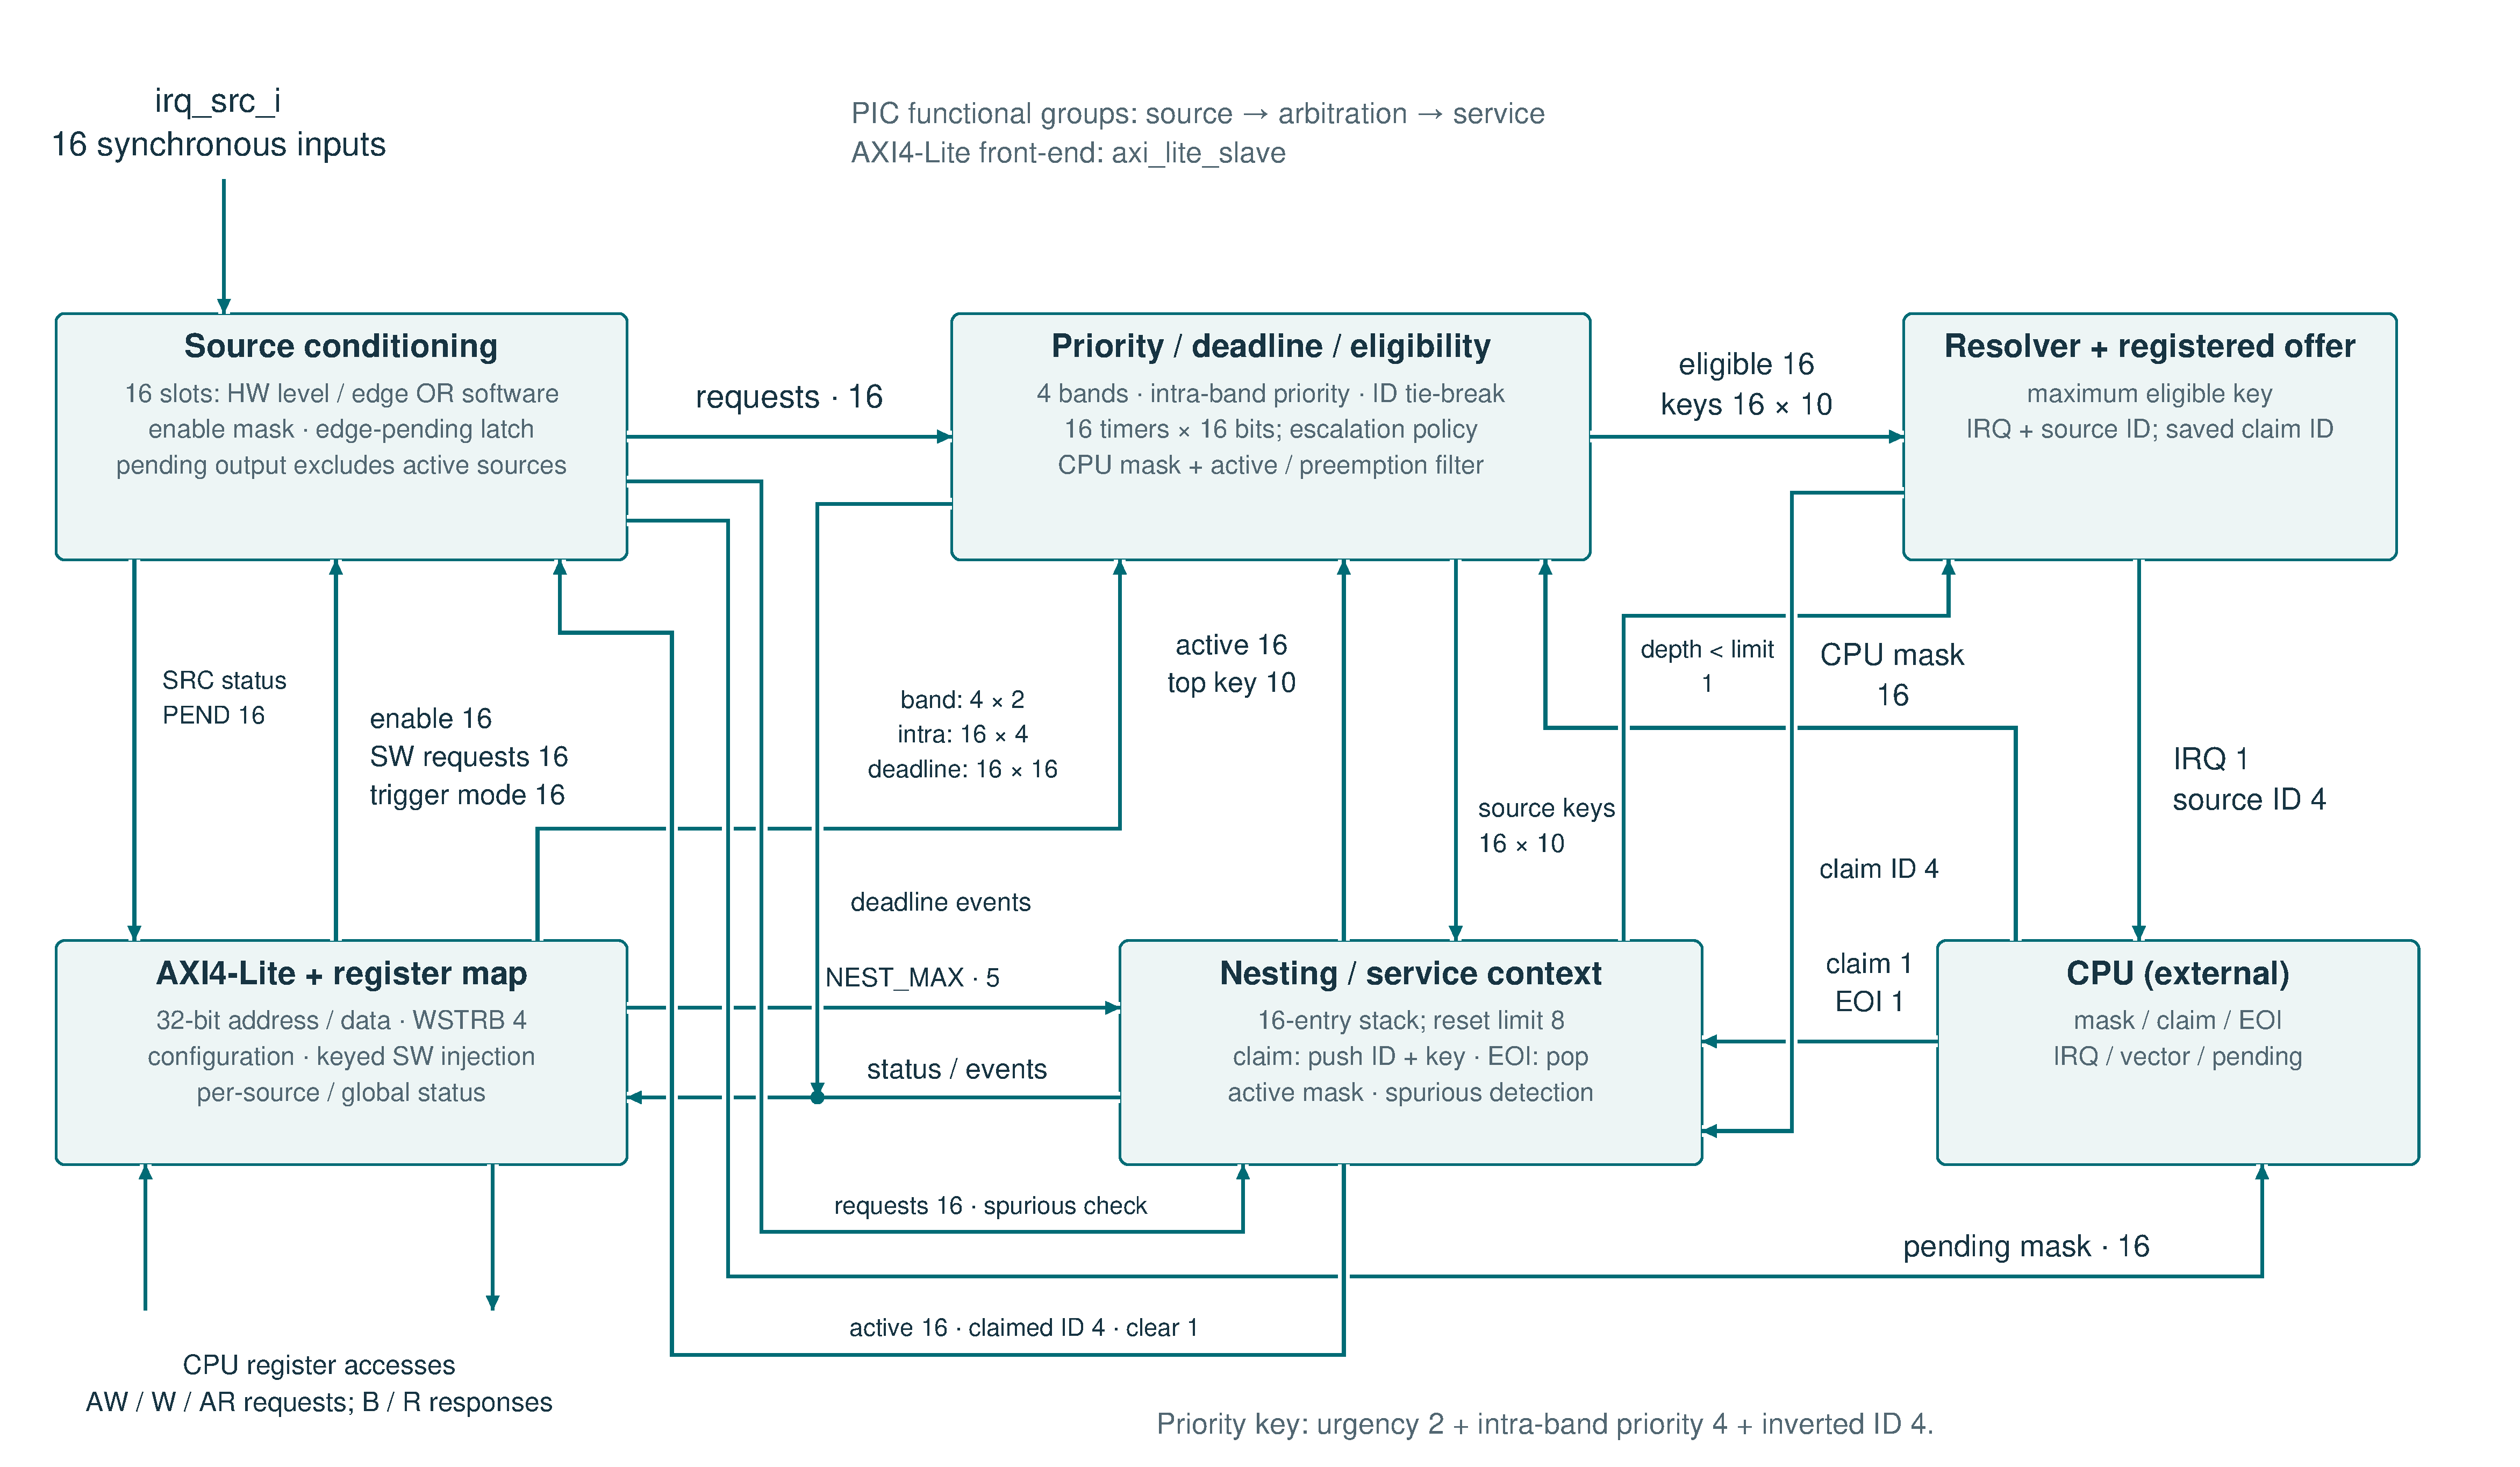
\includegraphics[width=\linewidth,height=132mm,keepaspectratio]{figures/pic_essential.pdf}\caption{Architectural view: HW/SW requests share 16 source slots; the stack records active service contexts.}\end{figure}

\end{landscape}
\restoregeometry
\sectionmark{Overview of overall structure}
\needspace{7\baselineskip}
\subsection{Arbitration and service contract}
\noindent Arbitration answers one question per cycle: which enabled source, if any, may be offered to the CPU. The table fixes how the winner is chosen, when a candidate may preempt an active context, and what the claim records.\par\medskip
{\small
\begin{longtable}{@{}L{0.2400\dimexpr\linewidth-12pt\relax}L{0.7600\dimexpr\linewidth-12pt\relax}@{}}
\toprule
\textbf{Decision} & \textbf{Contract} \\ \midrule
\endfirsthead
\toprule
\textbf{Decision} & \textbf{Contract} \\ \midrule
\endhead
Priority key & Band urgency first, then higher intra-band priority, then lower source ID. \\ \addlinespace[3pt]
Preemption & A candidate must be enabled, CPU-unmasked, inactive and strictly more urgent than the active top context. \\ \addlinespace[3pt]
Recorded context & Claim snapshots the selected source ID and priority. Reconfiguring an active source does not change that saved threshold. \\ \addlinespace[3pt]
Offer & cpu\_irq\_o and cpu\_irq\_vec\_o are registered together; pending\_o is a separate combinational mask. \\*
\bottomrule\end{longtable}}

\needspace{7\baselineskip}
\subsection{Source aggregation and offer timing}
\noindent The controller maintains one service identity per source slot. HW and SW requests for the same slot share configuration, priority, deadline and active state.\par\medskip
{\small
\begin{longtable}{@{}L{0.2500\dimexpr\linewidth-12pt\relax}L{0.7500\dimexpr\linewidth-12pt\relax}@{}}
\toprule
\textbf{Decision} & \textbf{Behaviour} \\ \midrule
\endfirsthead
\toprule
\textbf{Decision} & \textbf{Behaviour} \\ \midrule
\endhead
HW / SW collision & The enabled request is (selected HW level/latched edge OR SW pending). Simultaneous HW and SW activity produces one candidate, not two queued interrupt identities. \\ \addlinespace[3pt]
Pending storage & Edge and software requests use one pending bit per slot; repeated events before consumption coalesce. Level sources remain pending while the external line remains asserted. \\ \addlinespace[3pt]
Same-cycle events & A fresh edge wins over clearing the previous edge on claim. A keyed software set wins over the claim clear. After EOI, a retained request may be offered again. \\ \addlinespace[3pt]
Priority key & Four configurable 2-bit band urgencies, a per-source 4-bit intra-band priority, then inverted 4-bit ID. Select the largest key; lower source ID wins the final tie. \\ \addlinespace[3pt]
Reconfiguration & Changing an active source configuration affects future arbitration; the active stack entry keeps the key captured at claim until that context is popped. \\ \addlinespace[3pt]
Offer latency & Request conditioning and key comparison are combinational; IRQ/vector are registered at posedge. The claim consumes a one-cycle delayed copy of the offered vector. \\ \addlinespace[3pt]
Depth enforcement & Only an inactive, enabled, CPU-unmasked source above the saved top key is eligible. depth < NEST\_MAX is additionally required for an offer; an eligible blocked source sets OVF. \\*
\bottomrule\end{longtable}}

\needspace{7\baselineskip}
\subsection{Spurious and deadline policy}
\noindent The service decision uses the request state at claim. Deadline accounting covers enabled requests waiting for service, including requests masked at the CPU.\par\medskip
{\small
\begin{longtable}{@{}L{0.2500\dimexpr\linewidth-12pt\relax}L{0.7500\dimexpr\linewidth-12pt\relax}@{}}
\toprule
\textbf{Decision} & \textbf{Behaviour} \\ \midrule
\endfirsthead
\toprule
\textbf{Decision} & \textbf{Behaviour} \\ \midrule
\endhead
Spurious criterion & A claim is spurious when its saved source ID is no longer requested. Preserve the claimed service context, mark SRCx\_STATUS.SPUR, and set SPURIOUS\_LOG and INT\_STATUS.SPUR; EOI unwinds it normally. \\ \addlinespace[3pt]
Fast-clearing source & A level pulse gone before claim meets the same spurious criterion. Edge mode latches a pulse until claim and is the appropriate configuration when the event must survive deassertion. \\ \addlinespace[3pt]
Deadline storage / count & SRCx\_CONFIG[31:16] stores the 16-bit cycle deadline. Each slot counts while enabled pending and inactive; zero disables counting. CPU masking does not pause the timer. \\ \addlinespace[3pt]
Escalation & At deadline, either jump to the configured target band or select the next strictly greater programmed urgency. MULTI enables another escalation at each further deadline; the effective band cannot advance beyond the highest urgency. \\ \addlinespace[3pt]
After service / idle & On the first edge observing no wait, clear the counter and wait-local escalation flag and restore the configured band. Sticky INT\_STATUS.ESC remains until software clears it. \\ \addlinespace[3pt]
Software injection & Write 0xA5A50001 to SRCx\_SW\_TRIG with WSTRB[3:2]=11 and WSTRB[0]=1. Clear explicitly with bit 0=0, or automatically by claim. A software-only request follows the same deadline policy as hardware. \\*
\bottomrule\end{longtable}}

\needspace{7\baselineskip}
\subsection{Level request, claim and EOI}

\noindent Source 3 is offered and claimed once. Claim increases the active depth; after the source clears, EOI returns the controller to depth zero.\par
\begin{figure}[H]\centering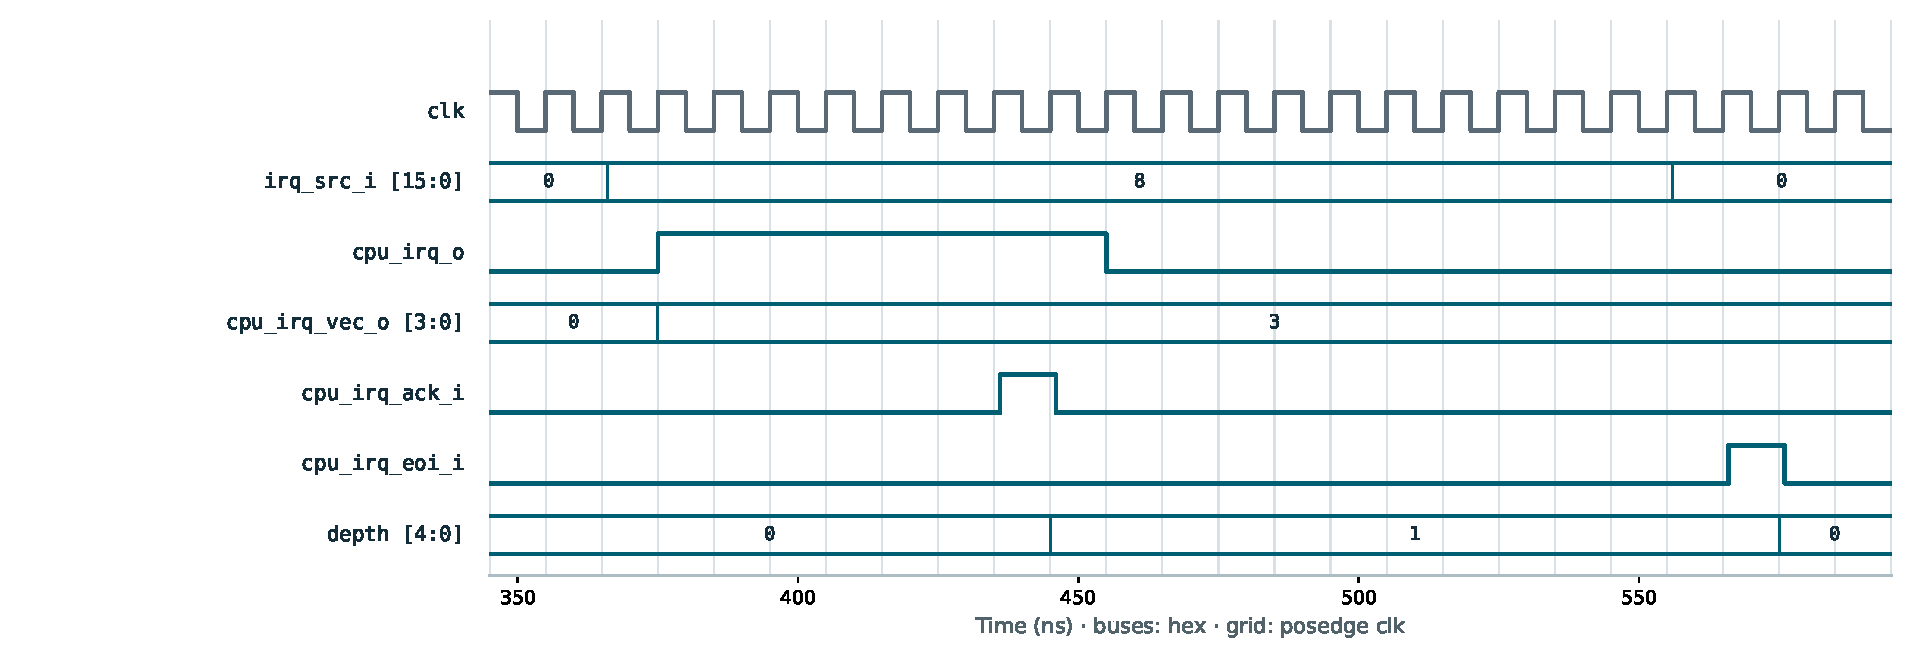
\includegraphics[width=\linewidth]{waves/pic_claim.pdf}\caption{Source 3 service: the request is claimed once; EOI returns nesting depth to zero.}\end{figure}
{\small
\begin{longtable}{@{}L{0.2800\dimexpr\linewidth-12pt\relax}L{0.7200\dimexpr\linewidth-12pt\relax}@{}}
\toprule
\textbf{Condition} & \textbf{Observable behaviour} \\ \midrule
\endfirsthead
\toprule
\textbf{Condition} & \textbf{Observable behaviour} \\ \midrule
\endhead
Enabled level high & Source becomes pending. cpu\_irq\_o is registered on the next resolution. \\ \addlinespace[3pt]
Claim & Push the previously offered source; mark it active; active sources are excluded from offers. \\ \addlinespace[3pt]
Source clears & The handler removes the peripheral cause before return. \\ \addlinespace[3pt]
EOI & Pop exactly one level. EOI on an empty stack is ignored. \\ \addlinespace[3pt]
Source remains high after EOI & It can become eligible again; PIC does not clear the external peripheral. \\*
\bottomrule\end{longtable}}

\needspace{7\baselineskip}
\subsection{Preemption and nesting}

\noindent Source 9 preempts source 8. The active mask keeps both sources during nesting; the first EOI restores source 8 and the second empties the stack. The offer vector is meaningful while cpu\_irq\_o is high.\par
\begin{figure}[H]\centering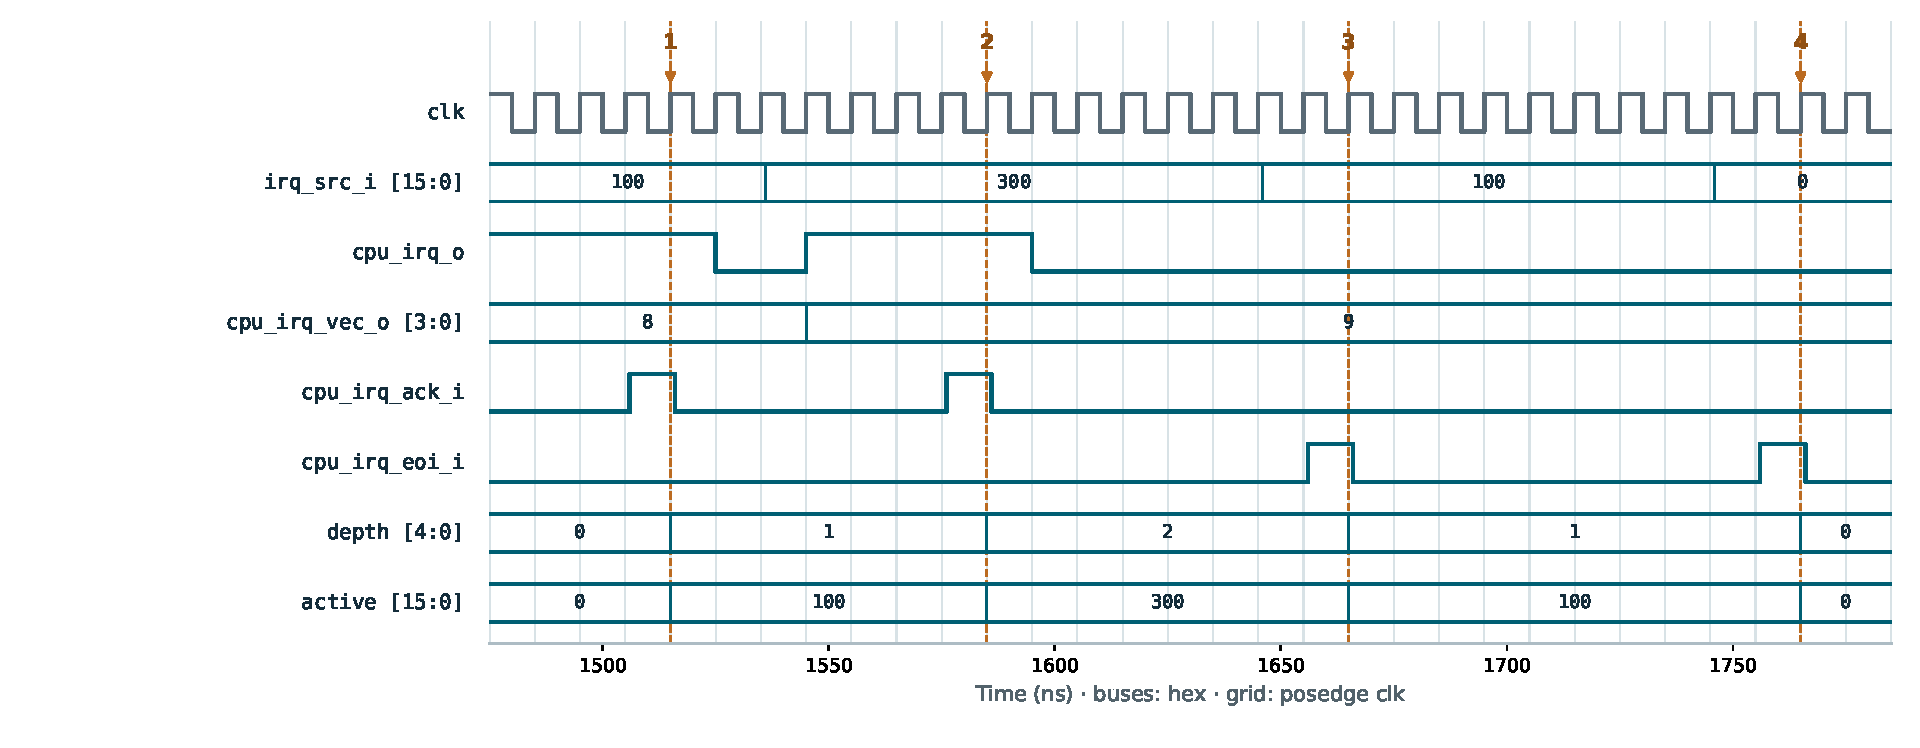
\includegraphics[width=\linewidth]{waves/pic_nesting.pdf}\caption{Source 8 enters service, source 9 preempts, and two EOIs restore then remove the outer context.}\end{figure}
{\small
\begin{longtable}{@{}L{0.2800\dimexpr\linewidth-12pt\relax}L{0.7200\dimexpr\linewidth-12pt\relax}@{}}
\toprule
\textbf{Condition} & \textbf{Result} \\ \midrule
\endfirsthead
\toprule
\textbf{Condition} & \textbf{Result} \\ \midrule
\endhead
Higher priority arrives & It may be offered while the current source is active. \\ \addlinespace[3pt]
Second claim & Depth increases from 1 to 2; outer source remains active. \\ \addlinespace[3pt]
Inner EOI & Depth returns to 1; outer priority threshold is restored. \\ \addlinespace[3pt]
At NEST\_MAX & No new offer; an eligible blocked source sets OVF. \\ \addlinespace[3pt]
Reband active source & Saved priority threshold is unchanged until that context is popped. \\*
\bottomrule\end{longtable}}

\needspace{7\baselineskip}
\subsection{Edge capture and spurious claims}

\noindent A second source edge is sampled with the claim of the first event. The edge latch remains set, and the source is offered again after EOI.\par
\begin{figure}[H]\centering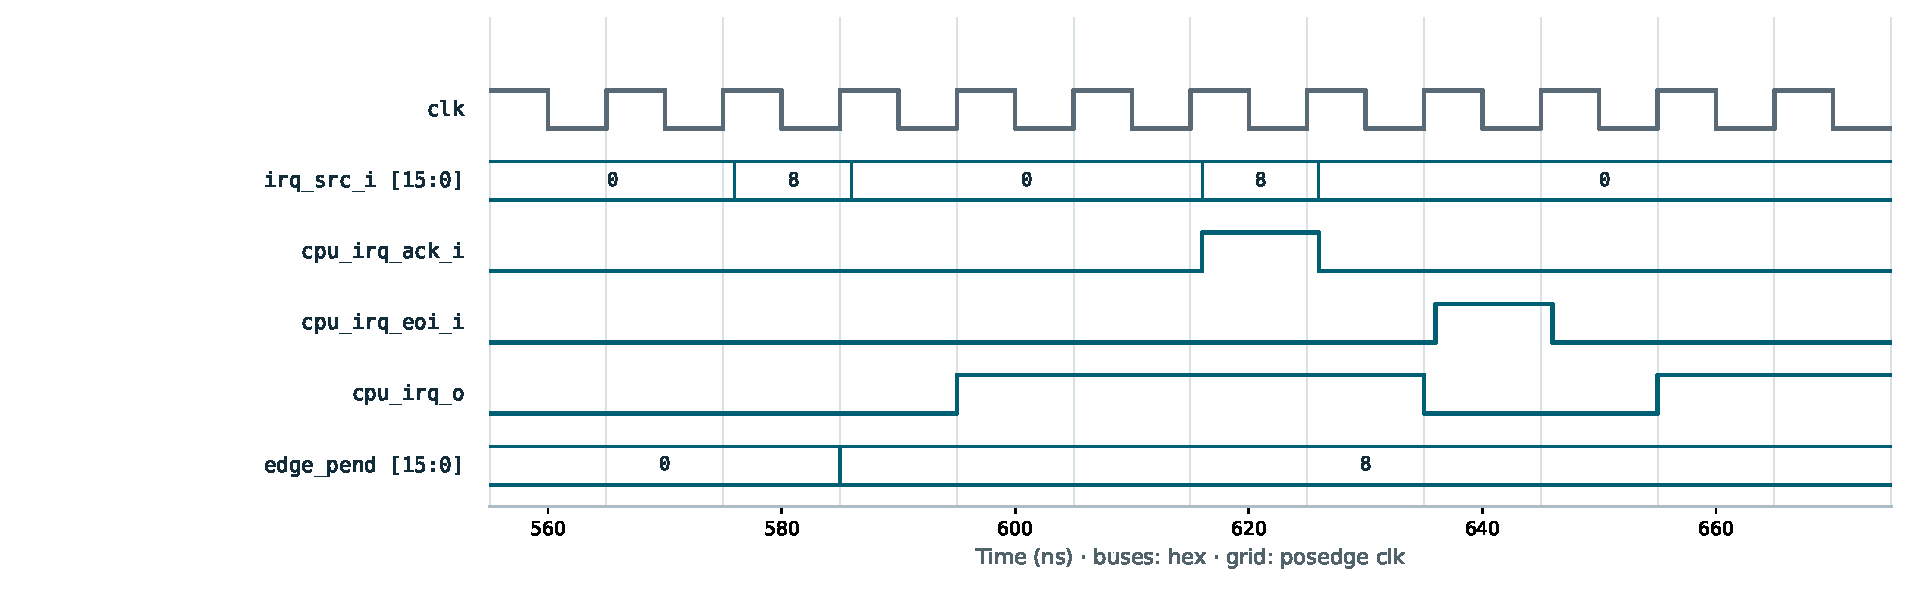
\includegraphics[width=\linewidth]{waves/pic_edge_claim.pdf}\caption{Simultaneous claim and a new source edge: the new edge remains latched for service after EOI.}\end{figure}

\noindent The level source disappears after its offer but before claim. The claim creates a service context marked spurious, allowing the CPU to unwind it through the same EOI sequence.\par
\begin{figure}[H]\centering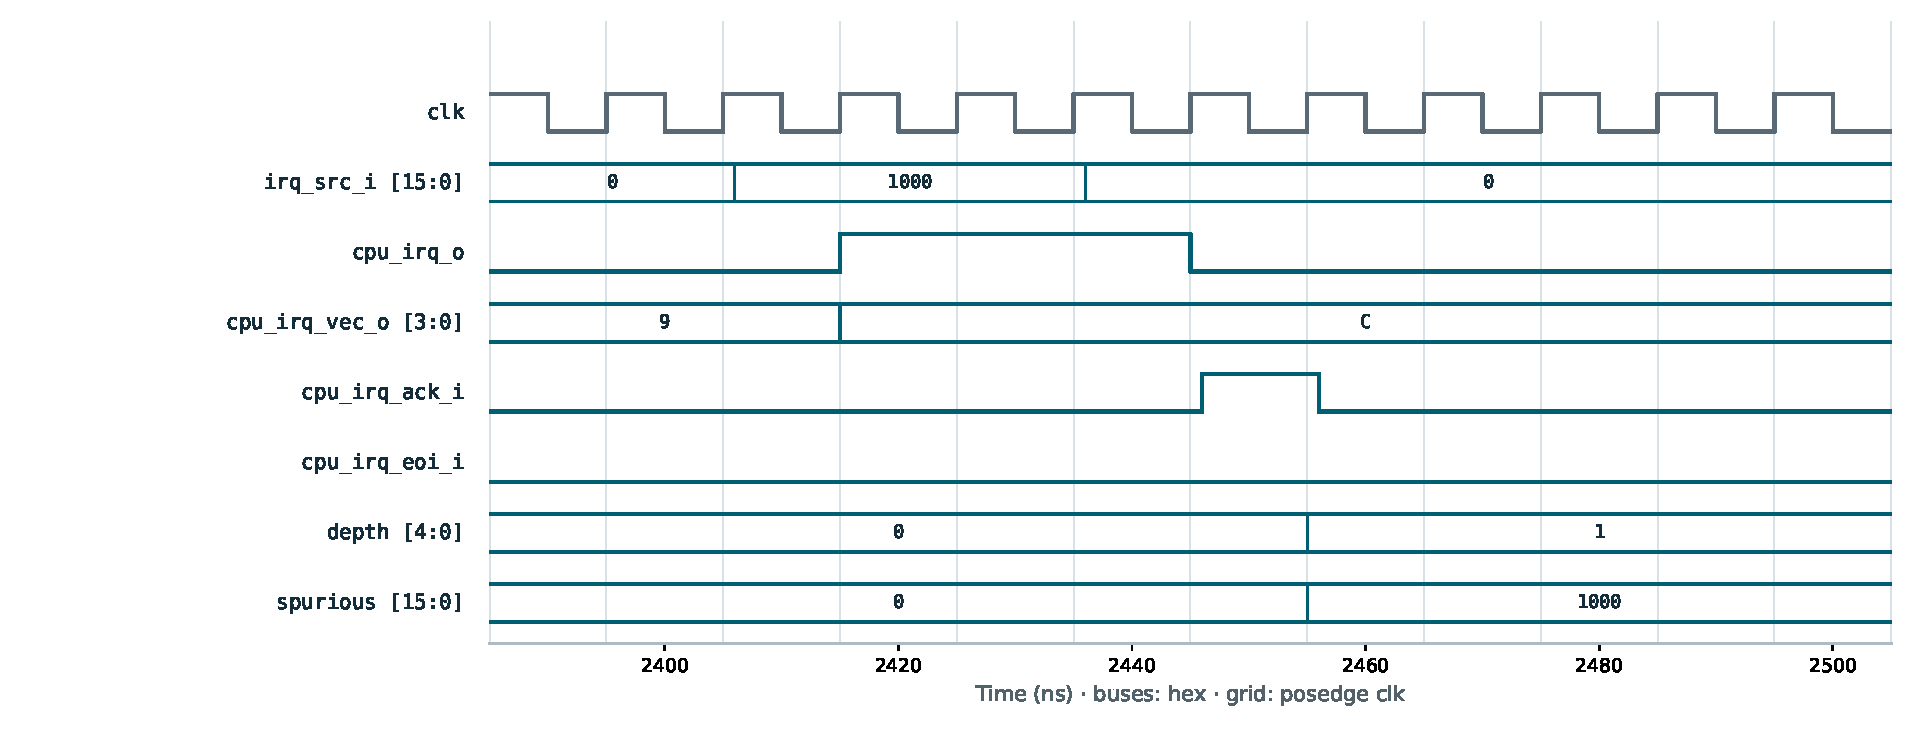
\includegraphics[width=\linewidth]{waves/pic_spurious.pdf}\caption{Source withdrawal before claim: the active context is marked spurious and the event is logged.}\end{figure}
{\small
\begin{longtable}{@{}L{0.2700\dimexpr\linewidth-12pt\relax}L{0.7300\dimexpr\linewidth-12pt\relax}@{}}
\toprule
\textbf{Event} & \textbf{Contract} \\ \midrule
\endfirsthead
\toprule
\textbf{Event} & \textbf{Contract} \\ \midrule
\endhead
Disabled edge source & A rising edge remains latched; enabling later exposes it. Level-mode reset slots capture no edges. \\ \addlinespace[3pt]
Claim with a new edge & New edge takes precedence over consuming the previous pending edge. \\ \addlinespace[3pt]
Spurious claim & The previously offered source is no longer pending when claimed; log globally and per source; unwind with normal EOI. \\*
\bottomrule\end{longtable}}

\needspace{7\baselineskip}
\subsection{Deadline escalation}

\noindent Source 1 initially wins the tie. Source 2 reaches its ten-cycle deadline; the escalation event changes its effective priority, and the registered offer changes to source 2 on the following edge.\par
\begin{figure}[H]\centering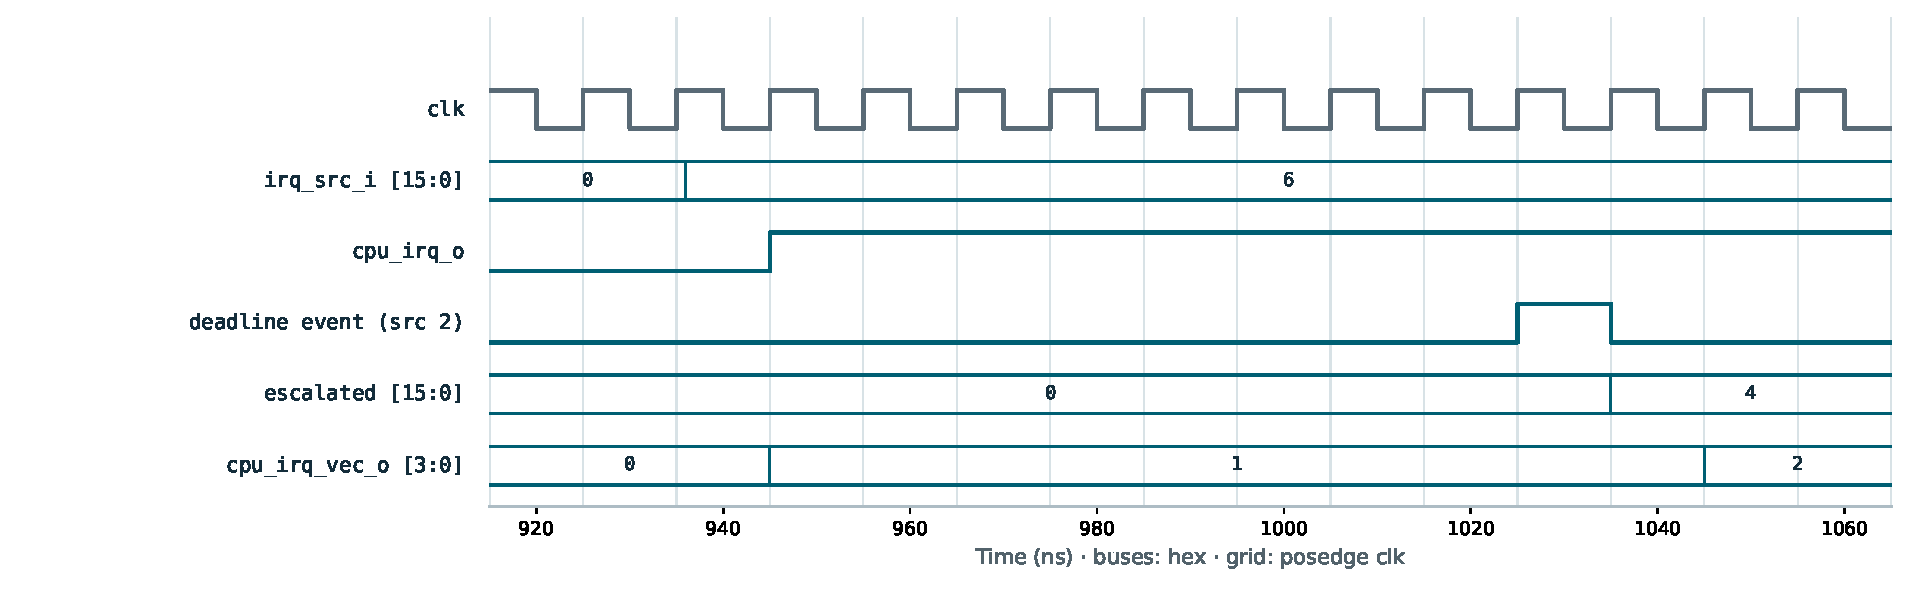
\includegraphics[width=\linewidth]{waves/pic_escalation.pdf}\caption{Reordered bands, source 2 deadline = 10 cycles: escalation precedes the registered offer changing from source 1 to 2.}\end{figure}
{\small
\begin{longtable}{@{}L{0.2900\dimexpr\linewidth-12pt\relax}L{0.7100\dimexpr\linewidth-12pt\relax}@{}}
\toprule
\textbf{Setting / event} & \textbf{Behaviour} \\ \midrule
\endfirsthead
\toprule
\textbf{Setting / event} & \textbf{Behaviour} \\ \midrule
\endhead
DEADLINE=0 & Timer disabled and held at zero. \\ \addlinespace[3pt]
Nonzero deadline & Count while enabled pending and not active. CPU masking does not stop the pending timer. \\ \addlinespace[3pt]
MODE=0 & Jump to TARGET when deadline expires. \\ \addlinespace[3pt]
MODE=1 & Move to the next strictly greater urgency in BAND\_CONFIG, which need not be the next lower band number. \\ \addlinespace[3pt]
MULTI=1 & Repeat at each deadline. In bump mode, the effective band stays unchanged if no higher urgency exists. \\ \addlinespace[3pt]
Claim / no longer pending & Clear elapsed wait and escalation state; configured priority applies again. \\ \addlinespace[3pt]
Status & SRCx\_STATUS.ESC is wait-local; INT\_STATUS.ESC is sticky until RW1C. \\*
\bottomrule\end{longtable}}

\clearpage
\section{Interfaces}
\subsection{Hardware interface}
\noindent All ports are digital and synchronous to the rising edge of clk\_i; rst\_n\_i is the only asynchronous input. The ports are the 16 source inputs, the CPU handshake (offer to the CPU, claim and EOI back) and the AXI4-Lite register port.\par\medskip
{\small
\begin{longtable}{@{}L{0.3400\dimexpr\linewidth-36pt\relax}L{0.1000\dimexpr\linewidth-36pt\relax}L{0.1000\dimexpr\linewidth-36pt\relax}L{0.4600\dimexpr\linewidth-36pt\relax}@{}}
\toprule
\textbf{Signal} & \textbf{Dir.} & \textbf{Width (bits)} & \textbf{Meaning} \\ \midrule
\endfirsthead
\toprule
\textbf{Signal} & \textbf{Dir.} & \textbf{Width (bits)} & \textbf{Meaning} \\ \midrule
\endhead
\texttt{clk\_i} & input & 1 & Rising-edge clock input. \\ \addlinespace[3pt]
\texttt{rst\_n\_i} & input & 1 & Asynchronous reset, active low. \\ \addlinespace[3pt]
\texttt{irq\_src\_i} & input & 16 & 16 synchronous hardware interrupt source lines. \\ \addlinespace[3pt]
\texttt{cpu\_mask\_i} & input & 16 & CPU acceptance mask, applied before priority selection. \\ \addlinespace[3pt]
\texttt{cpu\_irq\_o} & output & 1 & Registered interrupt offer; vector is valid while high. \\ \addlinespace[3pt]
\texttt{cpu\_irq\_vec\_o} & output & 4 & Registered offered source ID; meaningful while cpu\_irq\_o is high. \\ \addlinespace[3pt]
\texttt{pending\_o} & output & 16 & Enabled pending sources excluding active sources; independent of CPU mask. \\ \addlinespace[3pt]
\texttt{cpu\_irq\_ack\_i} & input & 1 & One-cycle claim of the previously sampled offer. \\ \addlinespace[3pt]
\texttt{cpu\_irq\_eoi\_i} & input & 1 & One-cycle end of interrupt; pop one active level. \\ \addlinespace[3pt]
\texttt{s\_axi\_awaddr\_i} & input & 32 & Write byte address. \\ \addlinespace[3pt]
\texttt{s\_axi\_awprot\_i} & input & 3 & Write protection attributes. \\ \addlinespace[3pt]
\texttt{s\_axi\_awvalid\_i} & input & 1 & Write address is valid; hold until handshake. \\ \addlinespace[3pt]
\texttt{s\_axi\_awready\_o} & output & 1 & Receiver can accept the write address. \\ \addlinespace[3pt]
\texttt{s\_axi\_wdata\_i} & input & 32 & Write payload. \\ \addlinespace[3pt]
\texttt{s\_axi\_wstrb\_i} & input & 4 & One enable bit per write byte. \\ \addlinespace[3pt]
\texttt{s\_axi\_wvalid\_i} & input & 1 & Write data is valid; hold until handshake. \\ \addlinespace[3pt]
\texttt{s\_axi\_wready\_o} & output & 1 & Receiver can accept the write data. \\ \addlinespace[3pt]
\texttt{s\_axi\_bresp\_o} & output & 2 & Write response: OKAY=00, SLVERR=10, DECERR=11. \\ \addlinespace[3pt]
\texttt{s\_axi\_bvalid\_o} & output & 1 & Write response is valid; hold until handshake. \\ \addlinespace[3pt]
\texttt{s\_axi\_bready\_i} & input & 1 & Receiver can accept the write response. \\ \addlinespace[3pt]
\texttt{s\_axi\_araddr\_i} & input & 32 & Read byte address. \\ \addlinespace[3pt]
\texttt{s\_axi\_arprot\_i} & input & 3 & Read protection attributes. \\ \addlinespace[3pt]
\texttt{s\_axi\_arvalid\_i} & input & 1 & Read address is valid; hold until handshake. \\ \addlinespace[3pt]
\texttt{s\_axi\_arready\_o} & output & 1 & Receiver can accept the read address. \\ \addlinespace[3pt]
\texttt{s\_axi\_rdata\_o} & output & 32 & Read payload. \\ \addlinespace[3pt]
\texttt{s\_axi\_rresp\_o} & output & 2 & Read response: OKAY=00, SLVERR=10, DECERR=11. \\ \addlinespace[3pt]
\texttt{s\_axi\_rvalid\_o} & output & 1 & Read response is valid; hold until handshake. \\ \addlinespace[3pt]
\texttt{s\_axi\_rready\_i} & input & 1 & Receiver can accept the read response. \\*
\bottomrule\end{longtable}}

\needspace{7\baselineskip}
\subsubsection{Reset and register-access contract}

\noindent The controller starts with active nested service and enabled sources. Reset clears both depth and INT\_ENABLE between clock edges; the test checks the state one nanosecond after assertion.\par
\begin{figure}[H]\centering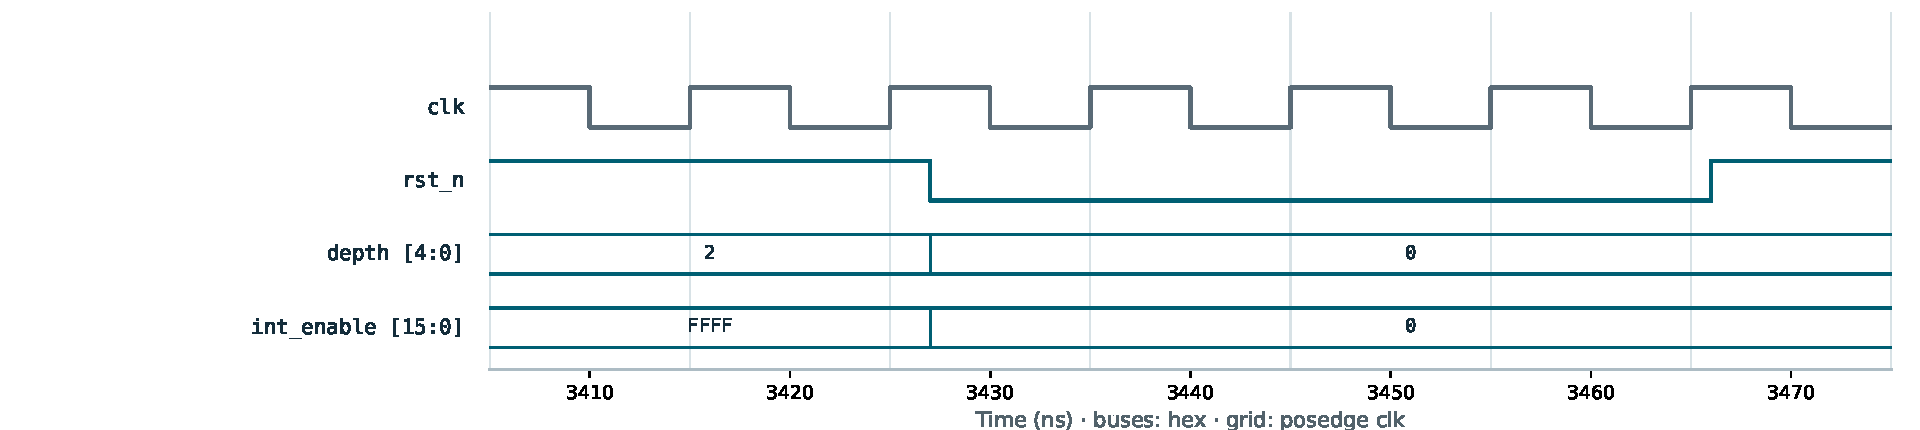
\includegraphics[width=\linewidth]{waves/pic_reset.pdf}\caption{Reset from a configured state: rst\_n asserts at posedge +2 ns; depth and enables clear before the next edge.}\end{figure}
{\small
\begin{longtable}{@{}L{0.2600\dimexpr\linewidth-12pt\relax}L{0.7400\dimexpr\linewidth-12pt\relax}@{}}
\toprule
\textbf{Item} & \textbf{Behaviour} \\ \midrule
\endfirsthead
\toprule
\textbf{Item} & \textbf{Behaviour} \\ \midrule
\endhead
Reset & Asynchronous active-low rst\_n\_i; sequential state updates on posedge clk\_i. \\ \addlinespace[3pt]
Reset state & INT\_ENABLE=0, depth=0, all source requests inactive; BAND\_CONFIG=0x1B, NEST\_MAX=8; other readable state zero. \\ \addlinespace[3pt]
Transactions & One outstanding read and one outstanding write. AW and W may arrive independently, in either order. \\ \addlinespace[3pt]
Read / write response & OKAY for a mapped permitted access. SLVERR for unmapped read/write or a write to RO. Rejected read data is zero. \\ \addlinespace[3pt]
Writes & WSTRB applies per byte as described in each field. No strobe does not authorize an otherwise forbidden write. \\ \addlinespace[3pt]
Reset during transfer & Captured AW/W and pending B/R responses are cleared; no pre-reset response is replayed afterwards. \\*
\bottomrule\end{longtable}}

\needspace{7\baselineskip}
\subsection{Software interface}
\noindent Every software-visible control and status bit of the controller lives in one 256-byte AXI4-Lite window. The map lists each offset with its access class and reset value; the subsections that follow give the fields of each register.\par\medskip
{\small
\begin{longtable}{@{}L{0.1700\dimexpr\linewidth-48pt\relax}L{0.2400\dimexpr\linewidth-48pt\relax}L{0.1300\dimexpr\linewidth-48pt\relax}L{0.1700\dimexpr\linewidth-48pt\relax}L{0.2900\dimexpr\linewidth-48pt\relax}@{}}
\toprule
\textbf{Byte offset} & \textbf{Name} & \textbf{Access type} & \textbf{Reset} & \textbf{Description} \\ \midrule
\endfirsthead
\toprule
\textbf{Byte offset} & \textbf{Name} & \textbf{Access type} & \textbf{Reset} & \textbf{Description} \\ \midrule
\endhead
0x00–0x3C & SRC0..15\_CONFIG & RW & 0x00000000 & Trigger, band, priority, deadline. \\ \addlinespace[3pt]
0x40–0x7C & SRC0..15\_SW\_TRIG & RW & 0x00000000 & Keyed injection / clear. \\ \addlinespace[3pt]
0x80–0xBC & SRC0..15\_STATUS & RO & 0x00000000 & Per-source state and timer. \\ \addlinespace[3pt]
0xC0 & BAND\_CONFIG & RW & 0x0000001B & Four urgency values. \\ \addlinespace[3pt]
0xC4 & NEST\_STATUS & RO & 0x00000000 & Depth, top ID and overflow. \\ \addlinespace[3pt]
0xC8 & NEST\_MAX & RW / WARL & 0x00000008 & Allowed active depth. \\ \addlinespace[3pt]
0xCC & ACTIVE\_VEC & RO & 0x00000000 & Active source and valid bit. \\ \addlinespace[3pt]
0xD0 & SPURIOUS\_LOG & RW1C & 0x00000000 & Per-source spurious flags. \\ \addlinespace[3pt]
0xD4 & ESCALATION\_CFG & RW & 0x00000000 & Escalation policy. \\ \addlinespace[3pt]
0xD8 & INT\_ENABLE & RW & 0x00000000 & Source enables. \\ \addlinespace[3pt]
0xDC & INT\_STATUS & RW1C & 0x00000000 & Global event flags. \\*
\bottomrule\end{longtable}}
{\small
\begin{longtable}{@{}L{0.2600\dimexpr\linewidth-12pt\relax}L{0.7400\dimexpr\linewidth-12pt\relax}@{}}
\toprule
\textbf{Rule} & \textbf{Meaning} \\ \midrule
\endfirsthead
\toprule
\textbf{Rule} & \textbf{Meaning} \\ \midrule
\endhead
Per-source offsets & x ranges from 0 to 15. Configuration=4x; software trigger=0x40+4x; status=0x80+4x. \\ \addlinespace[3pt]
Reserved addresses & 0xE0–0xFC return SLVERR. \\ \addlinespace[3pt]
Access classes & RW: read/write; RO: read-only; RW1C: write-one-to-clear; WARL: value coerced to a legal setting; RAZ/WI: read zero / write ignored. \\*
\bottomrule\end{longtable}}

\needspace{7\baselineskip}
\subsubsection{SRCx\_CONFIG — 0x00 + 4x}
{\small
\begin{longtable}{@{}L{0.1200\dimexpr\linewidth-48pt\relax}L{0.1800\dimexpr\linewidth-48pt\relax}L{0.1200\dimexpr\linewidth-48pt\relax}L{0.1200\dimexpr\linewidth-48pt\relax}L{0.4600\dimexpr\linewidth-48pt\relax}@{}}
\toprule
\textbf{Bits} & \textbf{Field} & \textbf{Access type} & \textbf{Reset} & \textbf{Description} \\ \midrule
\endfirsthead
\toprule
\textbf{Bits} & \textbf{Field} & \textbf{Access type} & \textbf{Reset} & \textbf{Description} \\ \midrule
\endhead
[31:16] & DEADLINE & RW & 0 & Pending cycles to escalation; zero disables the timer. \\ \addlinespace[3pt]
[15:8] & Reserved & RAZ/WI & 0 & Reads zero; writes ignored. \\ \addlinespace[3pt]
[7:4] & INTRA & RW & 0 & Higher value means higher priority within equal band urgency. \\ \addlinespace[3pt]
[3] & Reserved & RAZ/WI & 0 & Reads zero; writes ignored. \\ \addlinespace[3pt]
[2:1] & BAND & RW & 0 & Band index 0–3; urgency comes from BAND\_CONFIG. \\ \addlinespace[3pt]
[0] & TRIG & RW & 0 & 0: level. 1: latch rising edges until claim. \\*
\bottomrule\end{longtable}}

\needspace{7\baselineskip}
\subsubsection{SRCx\_SW\_TRIG — 0x40 + 4x}
{\small
\begin{longtable}{@{}L{0.1200\dimexpr\linewidth-48pt\relax}L{0.1800\dimexpr\linewidth-48pt\relax}L{0.1200\dimexpr\linewidth-48pt\relax}L{0.1200\dimexpr\linewidth-48pt\relax}L{0.4600\dimexpr\linewidth-48pt\relax}@{}}
\toprule
\textbf{Bits} & \textbf{Field} & \textbf{Access type} & \textbf{Reset} & \textbf{Description} \\ \midrule
\endfirsthead
\toprule
\textbf{Bits} & \textbf{Field} & \textbf{Access type} & \textbf{Reset} & \textbf{Description} \\ \midrule
\endhead
[31:16] & KEY & WO / RAZ & 0 & 0xA5A5 plus WSTRB[3:2]=11 is required to set SWREQ. \\ \addlinespace[3pt]
[15:1] & Reserved & RAZ/WI & 0 & Reads zero; writes ignored. \\ \addlinespace[3pt]
[0] & SWREQ & RW + HW clear & 0 & Set with key; zero clears without key. WSTRB[0] required. Claim clears; a simultaneous new set is retained. \\*
\bottomrule\end{longtable}}

\needspace{7\baselineskip}
\subsubsection{SRCx\_STATUS — 0x80 + 4x}
{\small
\begin{longtable}{@{}L{0.1200\dimexpr\linewidth-48pt\relax}L{0.1800\dimexpr\linewidth-48pt\relax}L{0.1200\dimexpr\linewidth-48pt\relax}L{0.1200\dimexpr\linewidth-48pt\relax}L{0.4600\dimexpr\linewidth-48pt\relax}@{}}
\toprule
\textbf{Bits} & \textbf{Field} & \textbf{Access type} & \textbf{Reset} & \textbf{Description} \\ \midrule
\endfirsthead
\toprule
\textbf{Bits} & \textbf{Field} & \textbf{Access type} & \textbf{Reset} & \textbf{Description} \\ \midrule
\endhead
[31:16] & DDL\_TIMER & RO & 0 & Elapsed enabled-pending cycles. Clears when idle or escalating; otherwise saturates at DEADLINE-1. \\ \addlinespace[3pt]
[15:6] & Reserved & RO & 0 & Reads zero. \\ \addlinespace[3pt]
[5:4] & EFF\_BAND & RO & 0 & Configured band, or temporary escalated band. \\ \addlinespace[3pt]
[3] & SPUR & RO & 0 & This active service level was claimed after its source disappeared. \\ \addlinespace[3pt]
[2] & ESC & RO & 0 & Escalated during the present wait; clears when claimed / no longer pending. \\ \addlinespace[3pt]
[1] & ACTIVE & RO & 0 & Source occupies a nesting level. \\ \addlinespace[3pt]
[0] & PEND & RO & 0 & Enabled HW/SW request, including a held level during its handler. \\*
\bottomrule\end{longtable}}

\needspace{7\baselineskip}
\subsubsection{BAND\_CONFIG — 0xC0}
{\small
\begin{longtable}{@{}L{0.1200\dimexpr\linewidth-48pt\relax}L{0.1800\dimexpr\linewidth-48pt\relax}L{0.1200\dimexpr\linewidth-48pt\relax}L{0.1200\dimexpr\linewidth-48pt\relax}L{0.4600\dimexpr\linewidth-48pt\relax}@{}}
\toprule
\textbf{Bits} & \textbf{Field} & \textbf{Access type} & \textbf{Reset} & \textbf{Description} \\ \midrule
\endfirsthead
\toprule
\textbf{Bits} & \textbf{Field} & \textbf{Access type} & \textbf{Reset} & \textbf{Description} \\ \midrule
\endhead
[31:8] & Reserved & RAZ/WI & 0 & Reads zero; writes ignored. \\ \addlinespace[3pt]
[7:6] & BAND3\_URG & RW & 0 & Urgency of band 3. \\ \addlinespace[3pt]
[5:4] & BAND2\_URG & RW & 1 & Urgency of band 2. \\ \addlinespace[3pt]
[3:2] & BAND1\_URG & RW & 2 & Urgency of band 1. \\ \addlinespace[3pt]
[1:0] & BAND0\_URG & RW & 3 & Urgency of band 0. Higher urgency wins. \\*
\bottomrule\end{longtable}}

\needspace{7\baselineskip}
\subsubsection{NEST\_STATUS — 0xC4}
{\small
\begin{longtable}{@{}L{0.1200\dimexpr\linewidth-48pt\relax}L{0.1800\dimexpr\linewidth-48pt\relax}L{0.1200\dimexpr\linewidth-48pt\relax}L{0.1200\dimexpr\linewidth-48pt\relax}L{0.4600\dimexpr\linewidth-48pt\relax}@{}}
\toprule
\textbf{Bits} & \textbf{Field} & \textbf{Access type} & \textbf{Reset} & \textbf{Description} \\ \midrule
\endfirsthead
\toprule
\textbf{Bits} & \textbf{Field} & \textbf{Access type} & \textbf{Reset} & \textbf{Description} \\ \midrule
\endhead
[31:17] & Reserved & RO & 0 & Reads zero. \\ \addlinespace[3pt]
[16] & OVF & RO & 0 & Alias of INT\_STATUS.OVF; clear at 0xDC. \\ \addlinespace[3pt]
[15:12] & Reserved & RO & 0 & Reads zero. \\ \addlinespace[3pt]
[11:8] & TOP\_ID & RO & 0 & Top active source ID; zero when depth is zero. \\ \addlinespace[3pt]
[7:5] & Reserved & RO & 0 & Reads zero. \\ \addlinespace[3pt]
[4:0] & DEPTH & RO & 0 & Active nesting levels, 0–16. \\*
\bottomrule\end{longtable}}

\needspace{7\baselineskip}
\subsubsection{NEST\_MAX — 0xC8}
{\small
\begin{longtable}{@{}L{0.1200\dimexpr\linewidth-48pt\relax}L{0.1800\dimexpr\linewidth-48pt\relax}L{0.1200\dimexpr\linewidth-48pt\relax}L{0.1200\dimexpr\linewidth-48pt\relax}L{0.4600\dimexpr\linewidth-48pt\relax}@{}}
\toprule
\textbf{Bits} & \textbf{Field} & \textbf{Access type} & \textbf{Reset} & \textbf{Description} \\ \midrule
\endfirsthead
\toprule
\textbf{Bits} & \textbf{Field} & \textbf{Access type} & \textbf{Reset} & \textbf{Description} \\ \midrule
\endhead
[31:5] & Reserved & RAZ/WI & 0 & Reads zero; writes ignored. \\ \addlinespace[3pt]
[4:0] & LIMIT & RW / WARL & 8 & Clamp 0 to 1 and values above 16 to 16. Requires WSTRB[0]. Lowering the limit does not unwind active handlers. \\*
\bottomrule\end{longtable}}

\needspace{7\baselineskip}
\subsubsection{ACTIVE\_VEC — 0xCC}
{\small
\begin{longtable}{@{}L{0.1200\dimexpr\linewidth-48pt\relax}L{0.1800\dimexpr\linewidth-48pt\relax}L{0.1200\dimexpr\linewidth-48pt\relax}L{0.1200\dimexpr\linewidth-48pt\relax}L{0.4600\dimexpr\linewidth-48pt\relax}@{}}
\toprule
\textbf{Bits} & \textbf{Field} & \textbf{Access type} & \textbf{Reset} & \textbf{Description} \\ \midrule
\endfirsthead
\toprule
\textbf{Bits} & \textbf{Field} & \textbf{Access type} & \textbf{Reset} & \textbf{Description} \\ \midrule
\endhead
[31:9] & Reserved & RO & 0 & Reads zero. \\ \addlinespace[3pt]
[8] & VALID & RO & 0 & At least one source is in service. \\ \addlinespace[3pt]
[7:4] & Reserved & RO & 0 & Reads zero. \\ \addlinespace[3pt]
[3:0] & ID & RO & 0 & Top active source; meaningful when VALID=1. \\*
\bottomrule\end{longtable}}

\needspace{7\baselineskip}
\subsubsection{SPURIOUS\_LOG — 0xD0}
{\small
\begin{longtable}{@{}L{0.1200\dimexpr\linewidth-48pt\relax}L{0.1800\dimexpr\linewidth-48pt\relax}L{0.1200\dimexpr\linewidth-48pt\relax}L{0.1200\dimexpr\linewidth-48pt\relax}L{0.4600\dimexpr\linewidth-48pt\relax}@{}}
\toprule
\textbf{Bits} & \textbf{Field} & \textbf{Access type} & \textbf{Reset} & \textbf{Description} \\ \midrule
\endfirsthead
\toprule
\textbf{Bits} & \textbf{Field} & \textbf{Access type} & \textbf{Reset} & \textbf{Description} \\ \midrule
\endhead
[31:16] & Reserved & RAZ/WI & 0 & Reads zero; writes ignored. \\ \addlinespace[3pt]
[15:0] & FLAGS & RW1C & 0 & One sticky bit per spurious source. WSTRB[1:0] qualify clear. New hardware set wins over clear. \\*
\bottomrule\end{longtable}}

\needspace{7\baselineskip}
\subsubsection{ESCALATION\_CFG — 0xD4}
{\small
\begin{longtable}{@{}L{0.1200\dimexpr\linewidth-48pt\relax}L{0.1800\dimexpr\linewidth-48pt\relax}L{0.1200\dimexpr\linewidth-48pt\relax}L{0.1200\dimexpr\linewidth-48pt\relax}L{0.4600\dimexpr\linewidth-48pt\relax}@{}}
\toprule
\textbf{Bits} & \textbf{Field} & \textbf{Access type} & \textbf{Reset} & \textbf{Description} \\ \midrule
\endfirsthead
\toprule
\textbf{Bits} & \textbf{Field} & \textbf{Access type} & \textbf{Reset} & \textbf{Description} \\ \midrule
\endhead
[31:9] & Reserved & RAZ/WI & 0 & Reads zero; writes ignored. \\ \addlinespace[3pt]
[8] & MULTI & RW & 0 & 1: repeat each deadline. 0: one escalation per wait. \\ \addlinespace[3pt]
[7:5] & Reserved & RAZ/WI & 0 & Reads zero; writes ignored. \\ \addlinespace[3pt]
[4] & MODE & RW & 0 & 0: jump to TARGET. 1: next strictly more urgent band. \\ \addlinespace[3pt]
[3:2] & Reserved & RAZ/WI & 0 & Reads zero; writes ignored. \\ \addlinespace[3pt]
[1:0] & TARGET & RW & 0 & Destination band for jump mode. \\*
\bottomrule\end{longtable}}

\needspace{7\baselineskip}
\subsubsection{INT\_ENABLE — 0xD8}
{\small
\begin{longtable}{@{}L{0.1200\dimexpr\linewidth-48pt\relax}L{0.1800\dimexpr\linewidth-48pt\relax}L{0.1200\dimexpr\linewidth-48pt\relax}L{0.1200\dimexpr\linewidth-48pt\relax}L{0.4600\dimexpr\linewidth-48pt\relax}@{}}
\toprule
\textbf{Bits} & \textbf{Field} & \textbf{Access type} & \textbf{Reset} & \textbf{Description} \\ \midrule
\endfirsthead
\toprule
\textbf{Bits} & \textbf{Field} & \textbf{Access type} & \textbf{Reset} & \textbf{Description} \\ \midrule
\endhead
[31:16] & Reserved & RAZ/WI & 0 & Reads zero; writes ignored. \\ \addlinespace[3pt]
[15:0] & ENABLE & RW & 0 & One source enable per bit; byte strobes apply. CPU mask is a separate filter. \\*
\bottomrule\end{longtable}}

\needspace{7\baselineskip}
\subsubsection{INT\_STATUS — 0xDC}
{\small
\begin{longtable}{@{}L{0.1200\dimexpr\linewidth-48pt\relax}L{0.1800\dimexpr\linewidth-48pt\relax}L{0.1200\dimexpr\linewidth-48pt\relax}L{0.1200\dimexpr\linewidth-48pt\relax}L{0.4600\dimexpr\linewidth-48pt\relax}@{}}
\toprule
\textbf{Bits} & \textbf{Field} & \textbf{Access type} & \textbf{Reset} & \textbf{Description} \\ \midrule
\endfirsthead
\toprule
\textbf{Bits} & \textbf{Field} & \textbf{Access type} & \textbf{Reset} & \textbf{Description} \\ \midrule
\endhead
[31:3] & Reserved & RAZ/WI & 0 & Reads zero; writes ignored. \\ \addlinespace[3pt]
[2] & OVF & RW1C & 0 & Eligible source blocked by depth limit. \\ \addlinespace[3pt]
[1] & ESC & RW1C & 0 & At least one deadline escalation occurred. \\ \addlinespace[3pt]
[0] & SPUR & RW1C & 0 & At least one spurious claim occurred. New hardware event wins over a same-cycle clear. \\*
\bottomrule\end{longtable}}

\needspace{7\baselineskip}
\subsubsection{Programming sequences}
\noindent A source is configured while it is disabled, enabled once its policy is set, then claimed and completed by the handler. The second table names the registers that make that state observable while the system is running.\par\medskip
{\small
\begin{longtable}{@{}L{0.0800\dimexpr\linewidth-24pt\relax}L{0.3400\dimexpr\linewidth-24pt\relax}L{0.5800\dimexpr\linewidth-24pt\relax}@{}}
\toprule
\textbf{Step} & \textbf{Register / signal} & \textbf{Action} \\ \midrule
\endfirsthead
\toprule
\textbf{Step} & \textbf{Register / signal} & \textbf{Action} \\ \midrule
\endhead
1 & INT\_ENABLE (0xD8) & Disable target source while configuring its trigger, band, intra priority and deadline. \\ \addlinespace[3pt]
2 & SRCx\_CONFIG (4x) & Write desired fields; set reserved bits to zero. \\ \addlinespace[3pt]
3 & BAND\_CONFIG / ESCALATION\_CFG / NEST\_MAX & Program shared policy as needed. \\ \addlinespace[3pt]
4 & INT\_ENABLE and cpu\_mask\_i & Enable source in PIC and permit it at CPU. \\ \addlinespace[3pt]
5 & SRCx\_SW\_TRIG (0x40+4x) & Set: WDATA=0xA5A50001 with WSTRB=0xD or 0xF. Clear: bit 0=0 with WSTRB[0]=1. \\ \addlinespace[3pt]
6 & cpu\_irq\_ack\_i & Claim one cycle after observing the offered request/vector. \\ \addlinespace[3pt]
7 & Peripheral / cpu\_irq\_eoi\_i & Clear the cause, then issue one EOI when the handler returns. \\ \addlinespace[3pt]
8 & INT\_STATUS / SPURIOUS\_LOG & Read events and write ones to the flags that should be cleared. \\*
\bottomrule\end{longtable}}
{\small
\begin{longtable}{@{}L{0.3800\dimexpr\linewidth-12pt\relax}L{0.6200\dimexpr\linewidth-12pt\relax}@{}}
\toprule
\textbf{Useful observation} & \textbf{Read} \\ \midrule
\endfirsthead
\toprule
\textbf{Useful observation} & \textbf{Read} \\ \midrule
\endhead
Pending / active / elapsed & SRCx\_STATUS. \\ \addlinespace[3pt]
Current handler & ACTIVE\_VEC.VALID and ID. \\ \addlinespace[3pt]
Nested contexts & NEST\_STATUS.DEPTH and TOP\_ID; software cannot read the whole stack. \\*
\bottomrule\end{longtable}}

\clearpage
\section{Reuse and reusability}
\noindent The one reused component is the register front end axi\_lite\_slave (section 6.1), which the machine timer also uses. Reusing the controller:\par\medskip
{\small
\begin{longtable}{@{}L{0.2500\dimexpr\linewidth-12pt\relax}L{0.7500\dimexpr\linewidth-12pt\relax}@{}}
\toprule
\textbf{Task} & \textbf{How to use this block} \\ \midrule
\endfirsthead
\toprule
\textbf{Task} & \textbf{How to use this block} \\ \midrule
\endhead
Compile & Include pic.v and axi\_lite\_slave.v. \\ \addlinespace[3pt]
Instantiate & pic has no Verilog module parameters; all configuration uses registers. \\ \addlinespace[3pt]
Connect & Map its 256-byte AXI window and connect 16 synchronous IRQ lines. Tie unused lines low. \\ \addlinespace[3pt]
CPU link & Connect request 1, vector 4, mask/pending 16 and claim/EOI 1 each. The original CPU brief differs; use the interface documented here. \\ \addlinespace[3pt]
Reset & Reset PIC, master and fabric together; keep a consistent reset domain for in-flight transactions. \\ \addlinespace[3pt]
Verify & Run the PIC benches in regress.do and the bound-assertion flow run\_verilator.sh; check the final address map. \\*
\bottomrule\end{longtable}}

\clearpage
\section{Design of submodules}
\noindent Submodule ports are synchronous to the rising edge of clk\_i and rst\_n\_i resets asynchronously; combinational modules have neither.\par\medskip
\addtocontents{toc}{\protect\setcounter{tocdepth}{2}}
\needspace{7\baselineskip}
\subsection{axi\_lite\_slave}
Collects independent AW/W channels and maps register-access acceptance to AXI response codes.
\subsubsection{Interface description}
\noindent No parameters.\par\medskip
{\small
\begin{longtable}{@{}L{0.3400\dimexpr\linewidth-36pt\relax}L{0.1000\dimexpr\linewidth-36pt\relax}L{0.1000\dimexpr\linewidth-36pt\relax}L{0.4600\dimexpr\linewidth-36pt\relax}@{}}
\toprule
\textbf{Signal} & \textbf{Dir.} & \textbf{Width (bits)} & \textbf{Meaning} \\ \midrule
\endfirsthead
\toprule
\textbf{Signal} & \textbf{Dir.} & \textbf{Width (bits)} & \textbf{Meaning} \\ \midrule
\endhead
\texttt{clk\_i} & input & 1 & Rising-edge clock input. \\ \addlinespace[3pt]
\texttt{rst\_n\_i} & input & 1 & Asynchronous reset, active low. \\ \addlinespace[3pt]
\texttt{s\_axi\_awaddr\_i} & input & 32 & Write byte address. \\ \addlinespace[3pt]
\texttt{s\_axi\_awvalid\_i} & input & 1 & Write address is valid; hold until handshake. \\ \addlinespace[3pt]
\texttt{s\_axi\_awready\_o} & output & 1 & Receiver can accept the write address. \\ \addlinespace[3pt]
\texttt{s\_axi\_wdata\_i} & input & 32 & Write payload. \\ \addlinespace[3pt]
\texttt{s\_axi\_wstrb\_i} & input & 4 & One enable bit per write byte. \\ \addlinespace[3pt]
\texttt{s\_axi\_wvalid\_i} & input & 1 & Write data is valid; hold until handshake. \\ \addlinespace[3pt]
\texttt{s\_axi\_wready\_o} & output & 1 & Receiver can accept the write data. \\ \addlinespace[3pt]
\texttt{s\_axi\_bresp\_o} & output & 2 & Write response: OKAY=00, SLVERR=10, DECERR=11. \\ \addlinespace[3pt]
\texttt{s\_axi\_bvalid\_o} & output & 1 & Write response is valid; hold until handshake. \\ \addlinespace[3pt]
\texttt{s\_axi\_bready\_i} & input & 1 & Receiver can accept the write response. \\ \addlinespace[3pt]
\texttt{s\_axi\_araddr\_i} & input & 32 & Read byte address. \\ \addlinespace[3pt]
\texttt{s\_axi\_arvalid\_i} & input & 1 & Read address is valid; hold until handshake. \\ \addlinespace[3pt]
\texttt{s\_axi\_arready\_o} & output & 1 & Receiver can accept the read address. \\ \addlinespace[3pt]
\texttt{s\_axi\_rdata\_o} & output & 32 & Read payload. \\ \addlinespace[3pt]
\texttt{s\_axi\_rresp\_o} & output & 2 & Read response: OKAY=00, SLVERR=10, DECERR=11. \\ \addlinespace[3pt]
\texttt{s\_axi\_rvalid\_o} & output & 1 & Read response is valid; hold until handshake. \\ \addlinespace[3pt]
\texttt{s\_axi\_rready\_i} & input & 1 & Receiver can accept the read response. \\ \addlinespace[3pt]
\texttt{wr\_en\_o} & output & 1 & Register write pulse after both AW and W have been collected. \\ \addlinespace[3pt]
\texttt{wr\_addr\_o} & output & 6 & Register word offset: captured AWADDR[7:2]. \\ \addlinespace[3pt]
\texttt{wr\_data\_o} & output & 32 & Captured write data. \\ \addlinespace[3pt]
\texttt{wr\_strb\_o} & output & 4 & Captured byte-lane enables. \\ \addlinespace[3pt]
\texttt{wr\_ok\_i} & input & 1 & Offset is writable; low selects SLVERR. Peripheral must qualify state updates. \\ \addlinespace[3pt]
\texttt{rd\_addr\_o} & output & 6 & Register word offset ARADDR[7:2]. \\ \addlinespace[3pt]
\texttt{rd\_data\_i} & input & 32 & Register read value for rd\_addr\_o. \\ \addlinespace[3pt]
\texttt{rd\_ok\_i} & input & 1 & Offset is readable; low selects SLVERR. \\*
\bottomrule\end{longtable}}
\subsubsection{Functional description}
\noindent AW and W are captured independently and one register-write pulse is issued after both are available. BRESP is retained until BREADY. An AR handshake samples the peripheral read mux and RRESP, which remain stable until RREADY. Register acceptance selects OKAY or SLVERR.\par\medskip

\addtocontents{toc}{\protect\setcounter{tocdepth}{3}}
\clearpage
\section{List of bugs and workarounds}
\noindent No open RTL defects are known at revision 2.2. Limitations that software and follow-up projects have to work around:\par\medskip
{\small
\begin{longtable}{@{}L{0.5000\dimexpr\linewidth-12pt\relax}L{0.5000\dimexpr\linewidth-12pt\relax}@{}}
\toprule
\textbf{Limitation} & \textbf{Workaround} \\ \midrule
\endfirsthead
\toprule
\textbf{Limitation} & \textbf{Workaround} \\ \midrule
\endhead
A level request that drops before the claim produces a spurious claim. & Use edge mode for short pulses. The handler reads SRCx\_STATUS.SPUR and still sends the EOI. \\ \addlinespace[3pt]
A software trigger needs WSTRB[3:2] and WSTRB[0]. & Arm it with a 32-bit store; byte and halfword stores cannot set a request. \\ \addlinespace[3pt]
Lowering NEST\_MAX below the current depth keeps the open levels. & Offers resume once EOIs bring the depth below the limit; change NEST\_MAX while no source is in service for immediate effect. \\*
\bottomrule\end{longtable}}

\end{document}
